\documentclass[UTF8]{ctexart}
\usepackage{amsmath}
\usepackage{amssymb}
\usepackage{graphicx}
\usepackage{hyperref}
\usepackage{geometry}
\usepackage{subcaption} 
\geometry{a4paper,left=2.5cm,right=2.5cm,top=2.5cm,bottom=2.5cm}

\begin{document}

\title{Lab3实验报告}
\author{倪煜晖 523030910170}
\date{\today}
\maketitle

\section{控制逻辑}
在Lab3 LC-3 Simulator的整个实现过程中,总体的控制逻辑没有使用新的全局变量,所有功能集成在process\_instruction()中实现。整体的控制逻辑如下:

\begin{enumerate}
    \item Fetch: 读取MEMORY[CURRENT\_LATCHES.PC],使用整型的instr存储读取到的指令,取出前四位存储到整型opcode中,具体实现方法在第二部分中说明。
    \item Decode:根据opcode的值决定执行的程序类型。
    \item Execute:根据ISA的要求执行对应指令操作寄存器、内存、条件码、PC等
\end{enumerate}
在实际实现中,使用的是switch-case语句,因此,实际上Decode和Execute可以说是一起实现的。
\section{功能实现}
注意到,LC3中,寄存器的容量与单条指令的长度均为16位,在用C实现的仿真器中,我们使用一个int变量就可以完成存储。这个性质是非常好的。所以,在之后的实现中
我们可以很方便的使用 \textbf{位运算}来大大简化运算。下面,列举几个关键功能的实现思路。

\subsection{Fetch and Decode}
\textbf{位操作与掩码的使用}是整个模拟器实现的核心思路。在Fetch and Decode中,
使用

{\centering int opcode = (instr $>>$ 12) \& 0xF \par}

取出前四位。之后,使用switch-case就可以简洁的处理分支跳转。

\subsection{取寄存器}
延续\textbf{位操作与使用掩码}的思路,只要把指令右移起始位置的位数加上掩码就可以读取到寄存器的值。以加法实现中DR的读取为例:

{\centering int dr = (instr $>>$ 9) \& 0x7 \par}

使用上面的指令,读取[11:9]处的DR值。

\subsection{取单个位}
取单个位在判断ADD,JSR,AND等指令的模式的时候十分重要,判断条件码的值也需要这个操作。它的实现思路仍然是\textbf{位操作与使用掩码}。
同样以ADD指令中的应用举例:

{\centering int imm\_flag = (instr $>>$ 5) \& 0x1 \par}

使用上面的指令获得了第5位的模式信息。以上,基本说明了取一位与多位的思路,后面的offset同样用这种方式得到,不再赘述。

\subsection{符号扩展}
为了实现正确的带符号运算,在运算前有时候要先实现符号扩展。使用三元运算符?:,配合掩码得到符号扩展的结果。以BR指令中的符号扩展为例:

{\centering  pc\_offset = (pc\_offset \& 0x100) ? (pc\_offset | 0xFE00) : pc\_offset \par}

BR指令采取的是offset9,用掩码0x100得到sign bit,再根据offset的正负进行对应扩展。

\subsection{操作数设置}
使用取单个位的方式取符号位。直接判断N与Z,用逻辑运算得到P
\begin{center}
          NEXT\_LATCHES.N = (result >> 15) \& 0x1;\\
      NEXT\_LATCHES.Z = (result == 0);\\
      NEXT\_LATCHES.P = !(NEXT\_LATCHES.N || NEXT\_LATCHES.Z);\\
\end{center}

\subsection{PC自增与跳转逻辑}
在LC3中,Fetch后PC直接自增,而我们的模拟程序使用CURRENT\_LATCHES与NEXT\_LATCHES记录状态。为了解决BR等指令中的offset实际上是在与自增后的PC做加法的问题,在适当的时候直接加一,最后再统一设置NEXT\_LATCHES.PC的值。


\section{验证与测试}
编译程序,编写测试shell,按照要求编译运行:

\begin{figure}[htbp!]
    \centering
    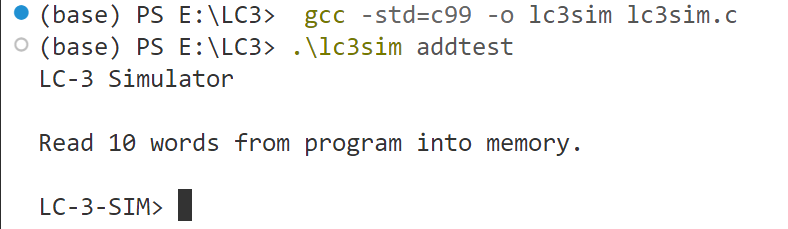
\includegraphics[width=0.8\textwidth]{launch.png}
    \caption{LC3 Simulator启动}
\end{figure}

\subsection{ADD功能测试}
执行以下命令:
\begin{enumerate}
    \item[ ] .ORIG 0x3000 (0x3000)
    \item[0x3000] ADD R0,R0,\#1 (0x1021)
    \item[0x3001]  ADD R1,R1,\#3 (0x1263)
    \item[0x3002]  ADD R1,R1,\#-1(0x127F)
    \item[0x3003] ADD R2,R0,R1(0x1401)
    \item[0x3004] ADD R4,R4,\#-1(0x193F)
\end{enumerate}

运行结果如图\ref{ADD}.

可以看到,第一、二条指令验证了立即数模式的正确性,第三条验证了加负数功能的正确性,第四条验证了寄存器模式的正确性,最后一条说明 Low16bits(x) ((x) \& 0xFFFF)的处理方式运行正常。此外,各指令均正确处理了条件码。
\begin{figure}[htbp]
  \centering
  \begin{subfigure}{0.45\textwidth}
    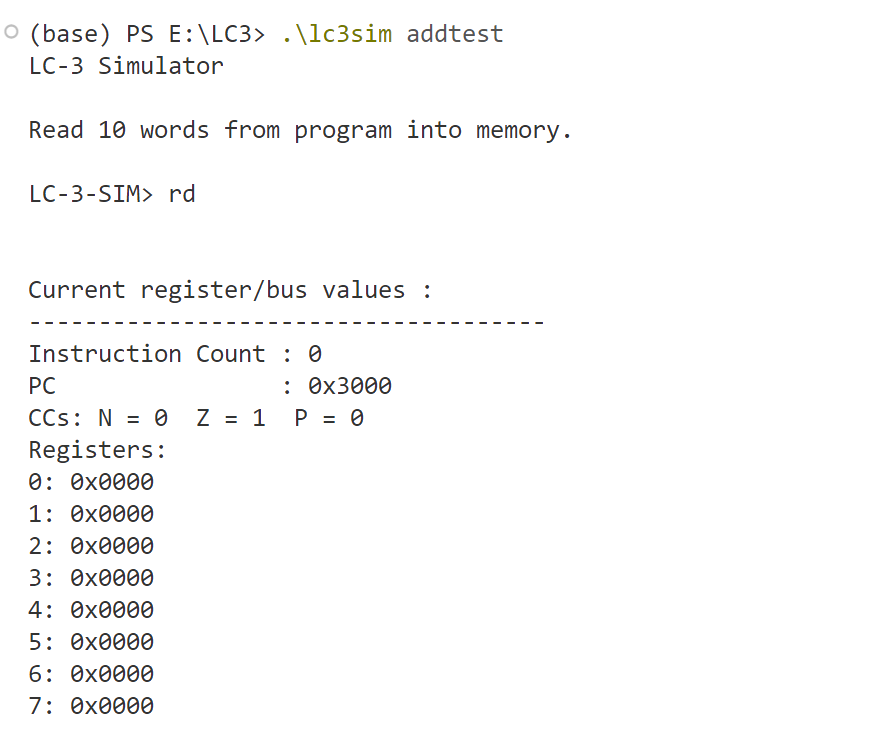
\includegraphics[width=\linewidth]{add1.png}
    \caption{图1}
  \end{subfigure}
  \hfill
  \begin{subfigure}{0.45\textwidth}
    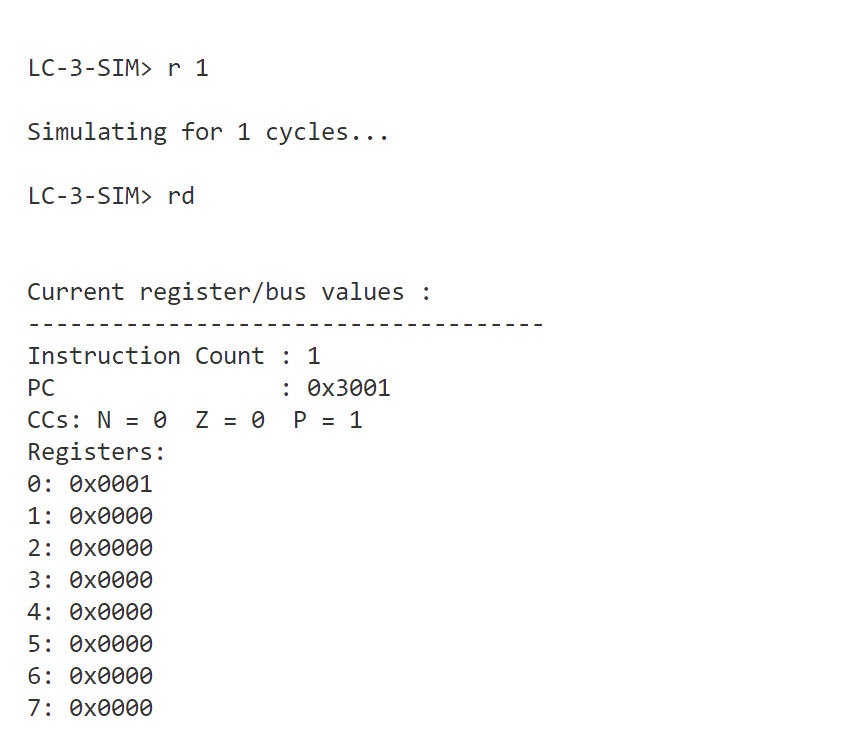
\includegraphics[width=\linewidth]{add2.png}
    \caption{图2}
  \end{subfigure}

  \vspace{0.5cm}

  \begin{subfigure}{0.45\textwidth}
    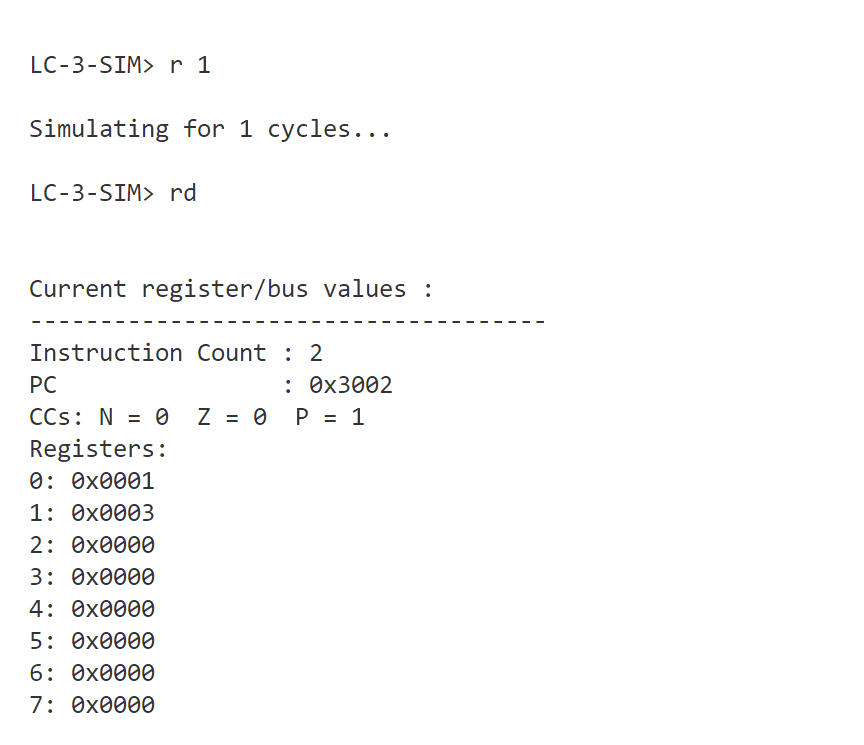
\includegraphics[width=\linewidth]{add3.png}
    \caption{图3}
  \end{subfigure}
  \hfill
  \begin{subfigure}{0.45\textwidth}
    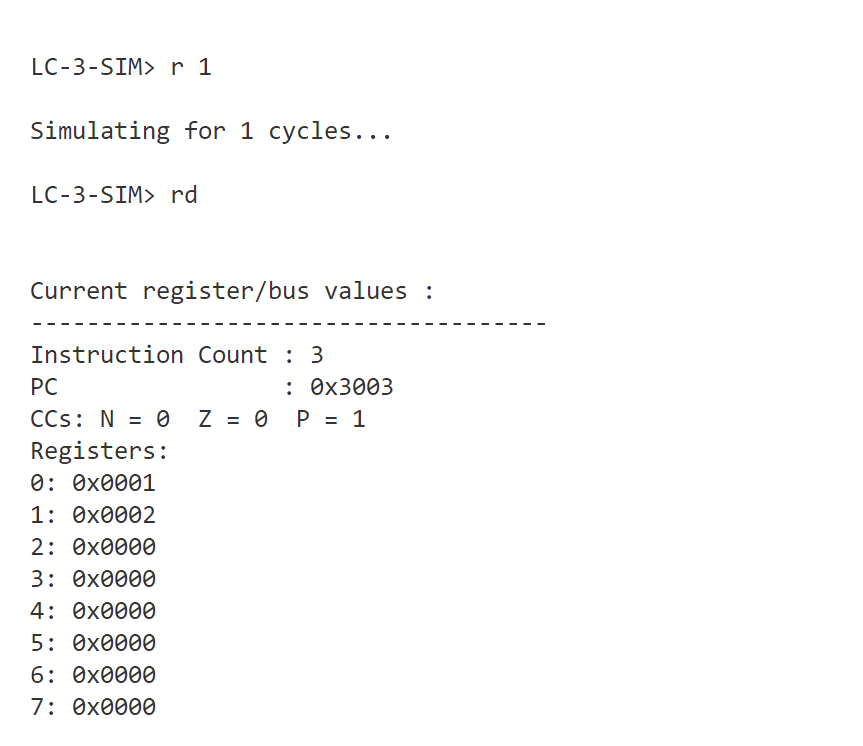
\includegraphics[width=\linewidth]{add4.png}
    \caption{图4}
  \end{subfigure}

  \vspace{0.5cm}

  \begin{subfigure}{0.45\textwidth}
    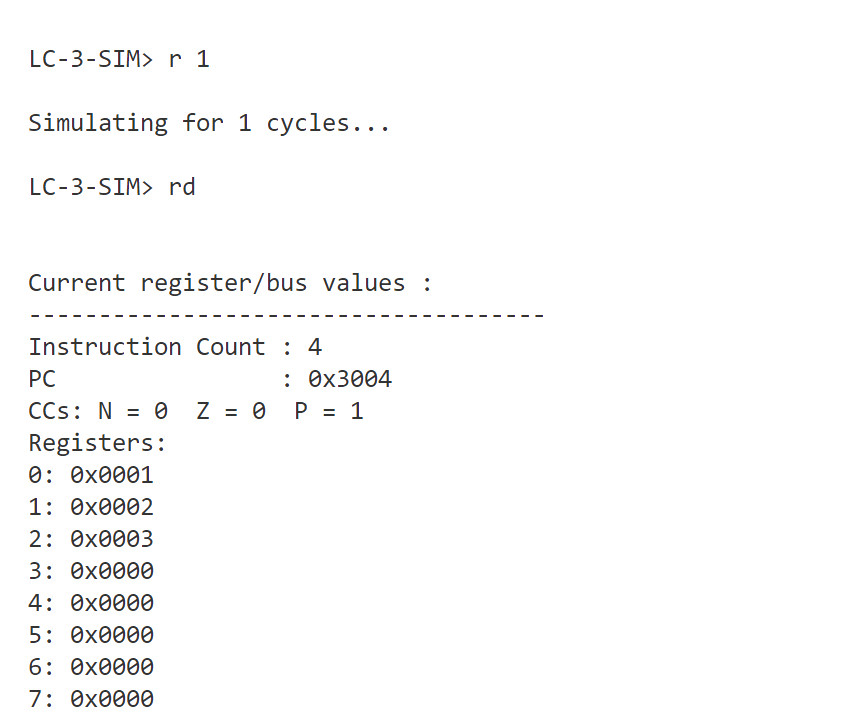
\includegraphics[width=\linewidth]{add5.png}
    \caption{图5}
  \end{subfigure}
  \hfill
  \begin{subfigure}{0.45\textwidth}
    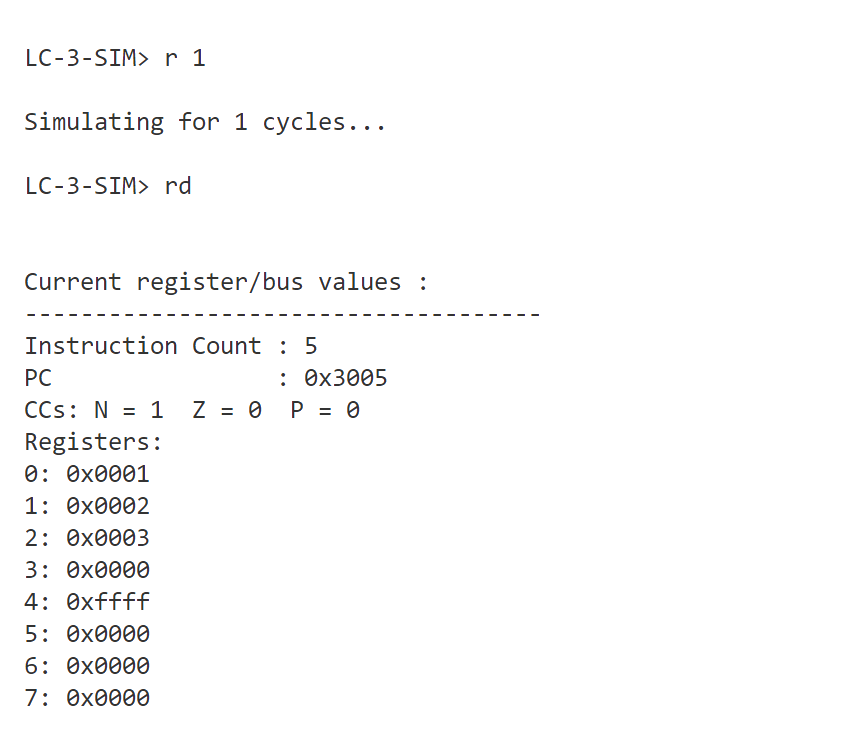
\includegraphics[width=\linewidth]{add6.png}
    \caption{图6}
  \end{subfigure}

  \caption{ADD功能测试}
  \label{ADD}
\end{figure}

\subsection{NOT功能测试}
在之前程序的基础上继续执行:
\begin{enumerate}
    \item[0x3005] NOT R3,R3(0x96FF)
\end{enumerate}
运行结果如图\ref{not}.

可见,程序正确把0x0000反转为0xFFFF并且正确设置条件码。
\begin{figure}[htbp]
  \centering
  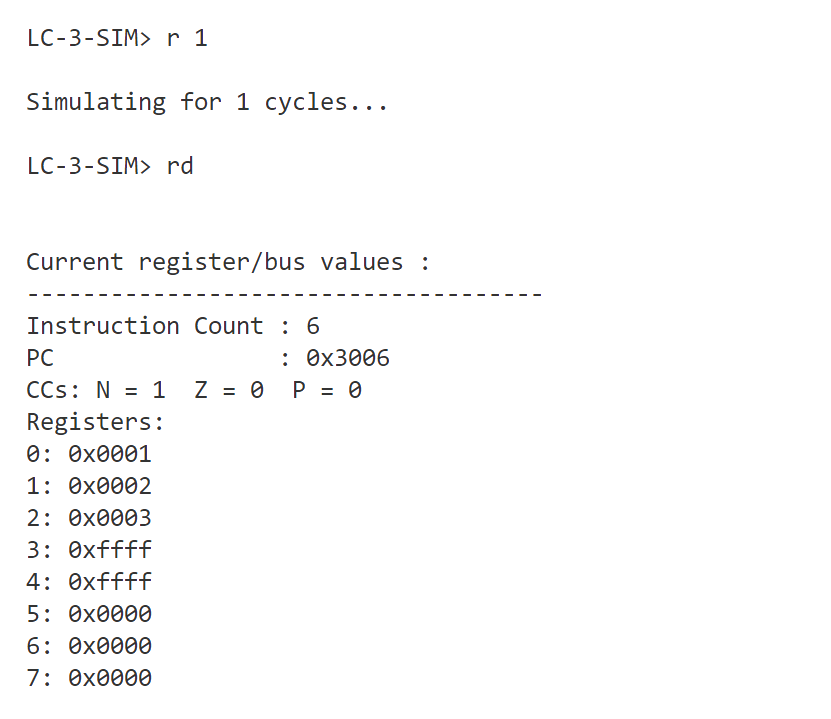
\includegraphics[width=0.8\textwidth]{not.png} % 替换为你的图片路径
  \caption{NOT功能测试}
  \label{not}
\end{figure}

\subsection{AND功能测试}
在之前程序的基础上继续执行:
\begin{enumerate}
    \item[0x3006] AND R5,R0,R1(0x5A01)
    \item[0x3007]AND R5,R1,\#2(0x5AA2)
\end{enumerate}
运行结果如图\ref{and}.

程序在寄存器模式与立即数模式下均正常运行并且正确设置条件码。
\begin{figure}[htbp]
  \centering
  \begin{subfigure}{0.48\textwidth} % 留出间距
    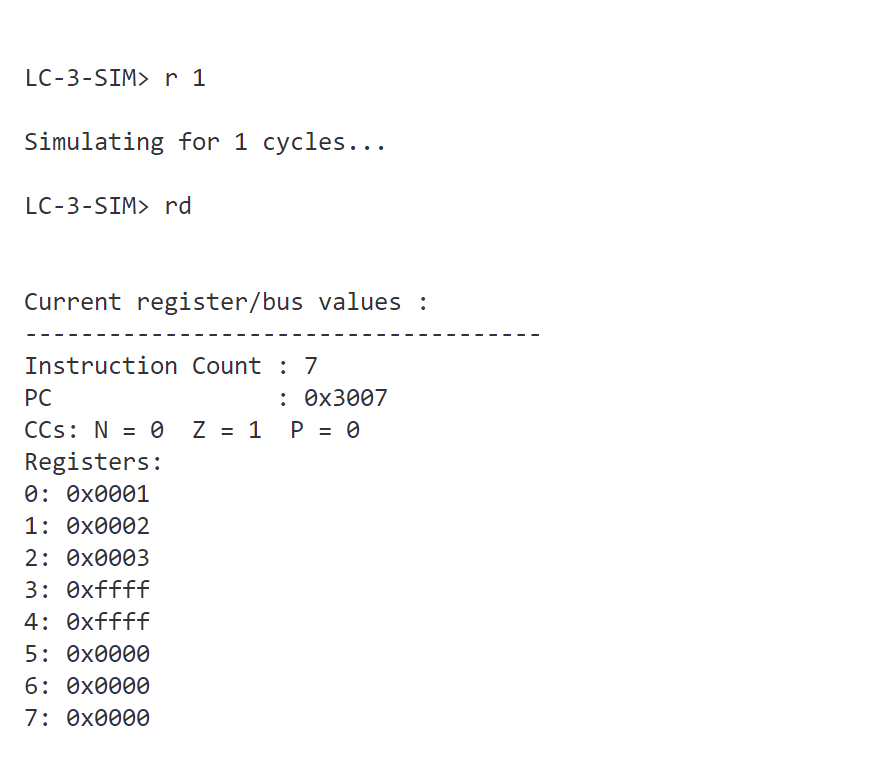
\includegraphics[width=\linewidth]{and1.png}
    \caption{寄存器模式}
  \end{subfigure}
  \hfill
  \begin{subfigure}{0.48\textwidth}
    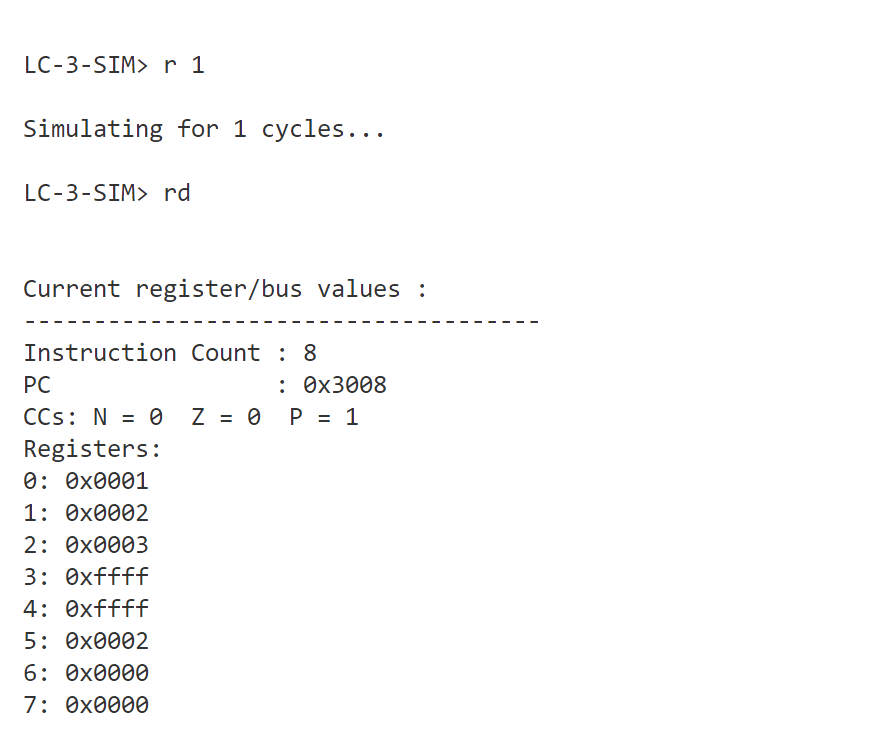
\includegraphics[width=\linewidth]{and2.png}
    \caption{立即数模式}
  \end{subfigure}
  \caption{AND功能测试}
  \label{and}
\end{figure}


\subsection{BR功能测试}
在之前程序的基础上继续执行:
\begin{enumerate}
    \item[0x3008] BRN \#4(0x0804)
    \item[0x3009]BRP \#4(0x0204)
\end{enumerate}
运行结果如图\ref{br}.

在上一条AND后,N=0,Z=0,P=1,所以BRN不做任何事情,BRP正确跳转到自增后PC+offset的位置。
\begin{figure}[htbp]
  \centering
  \begin{subfigure}{0.48\textwidth} % 留出间距
    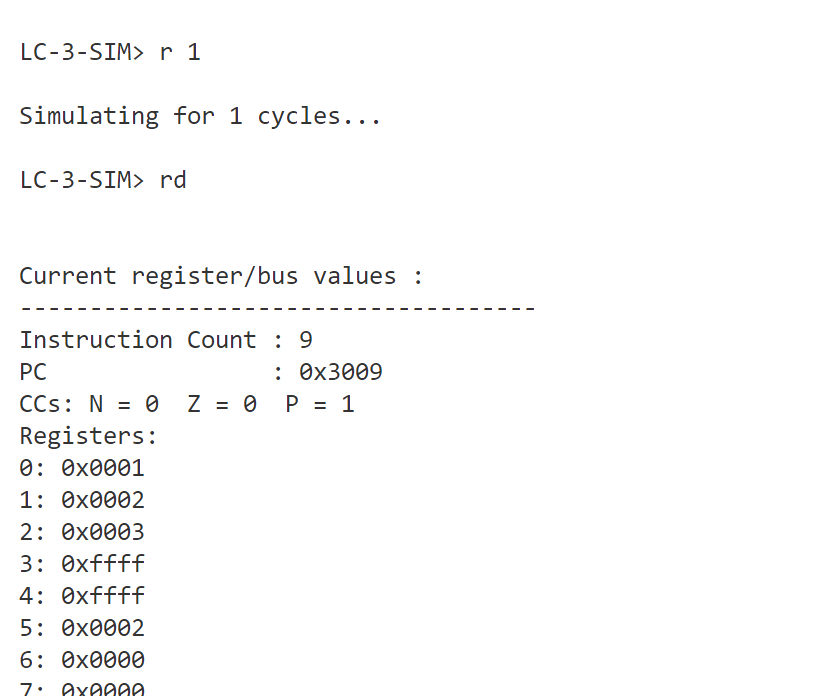
\includegraphics[width=\linewidth]{br1.png}
    \caption{不跳转}
  \end{subfigure}
  \hfill
  \begin{subfigure}{0.48\textwidth}
    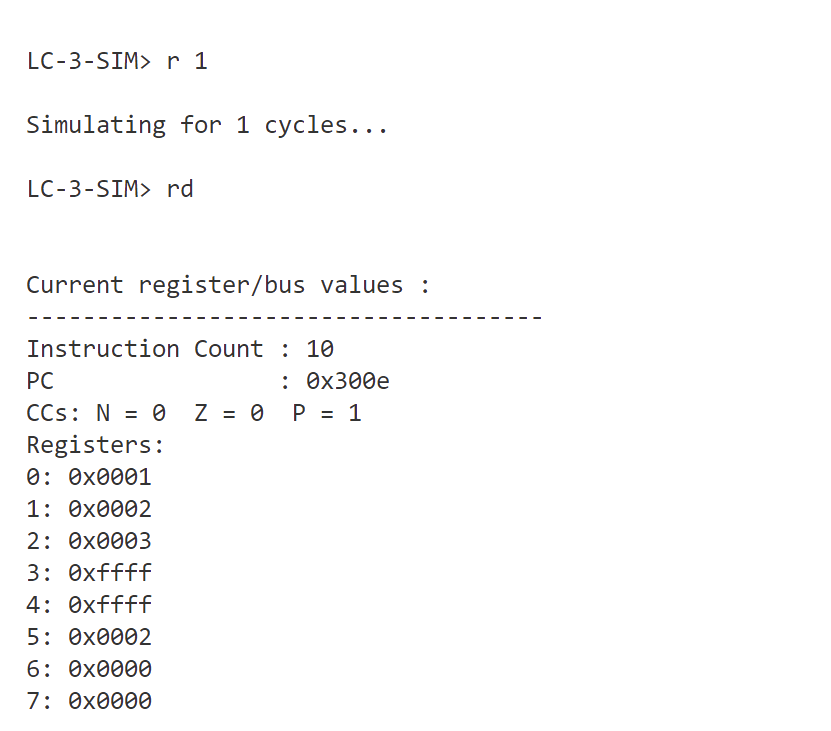
\includegraphics[width=\linewidth]{br2.png}
    \caption{跳转}
  \end{subfigure}
  \caption{BR功能测试}
  \label{br}
\end{figure}

\subsection{TRAP功能测试}
运行如下代码:
\begin{enumerate}
    \item[ ] .ORIG 0x3000 (0x3000)
    \item[0x3000] TRAP x25(0xF025)
\end{enumerate}
运行结果如图\ref{trap}.

程序正确保存PC到R7.由于全部初始化为0,所以无论TRAP什么,都会跳转到0x0000然后触发HALT。
\begin{figure}[htbp]
  \centering
  \begin{subfigure}{0.48\textwidth} % 留出间距
    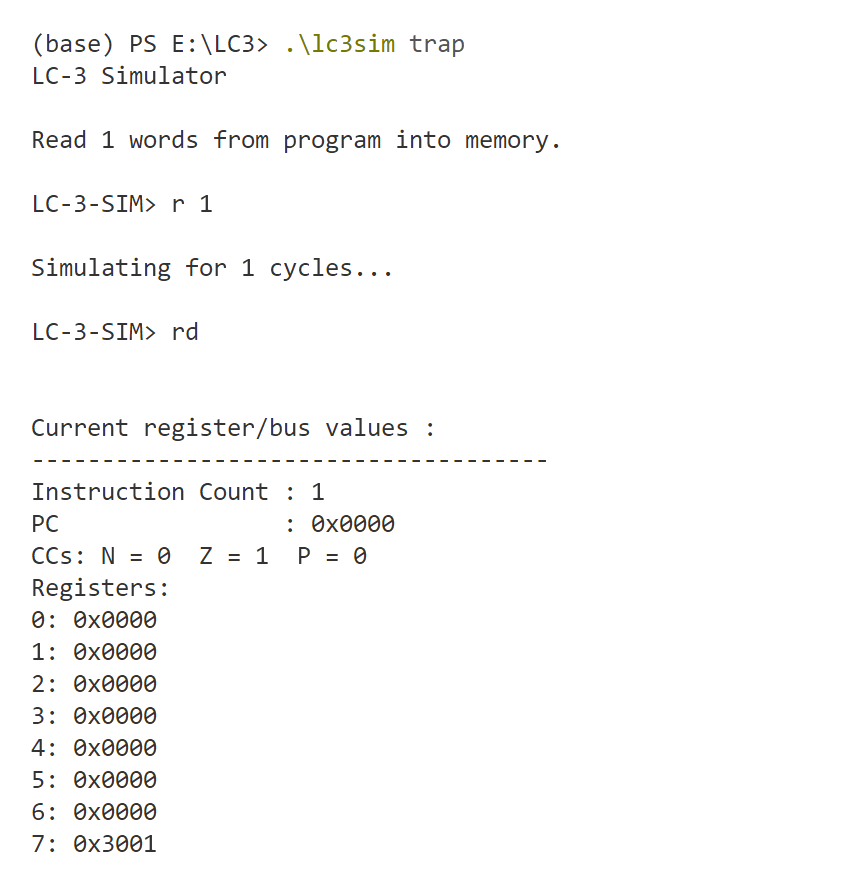
\includegraphics[width=\linewidth]{trap1.png}
  \end{subfigure}
  \hfill
  \begin{subfigure}{0.48\textwidth}
    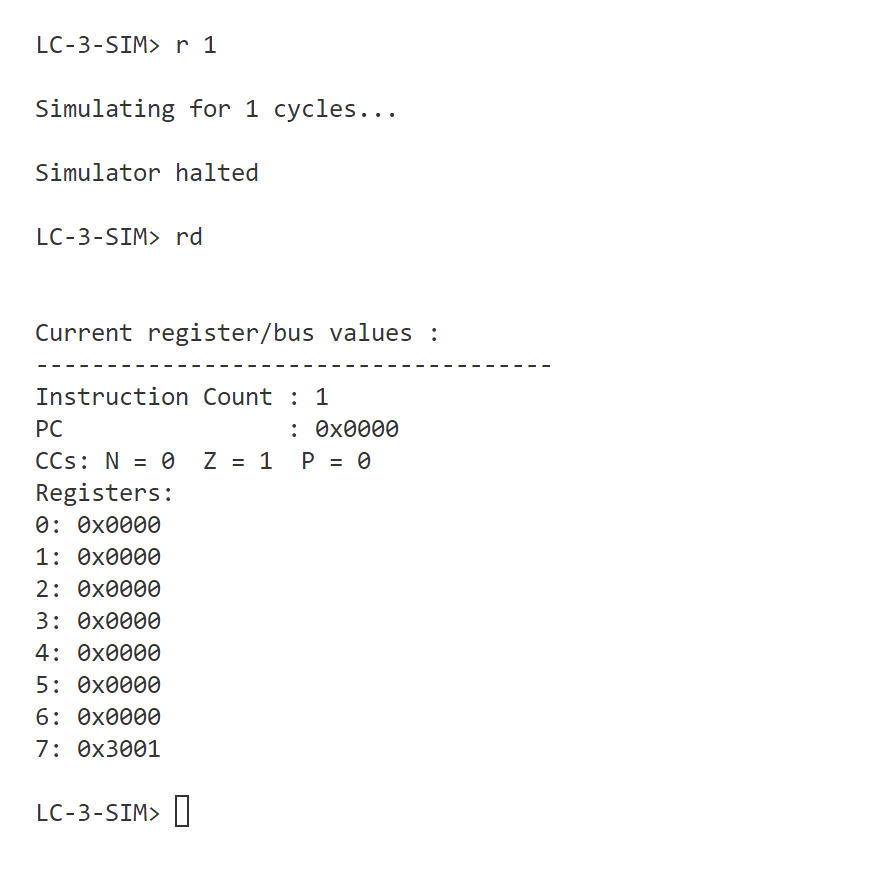
\includegraphics[width=\linewidth]{trap2.png}
  \end{subfigure}
  \caption{TRAP功能测试}
  \label{trap}
\end{figure}

\subsection{LEA与JMP功能测试}
运行如下代码:
\begin{enumerate}
  \item [ ] .ORIG 0x3000
  \item [0x3000] LEA R0,\# -1(0xE1FF)
  \item [0x3001] JMP R0(0xC000)
\end{enumerate}
运行结果如图\ref{leajmp}:
\begin{figure}[htbp]
  \centering
  \begin{subfigure}{0.48\textwidth} % 留出间距
    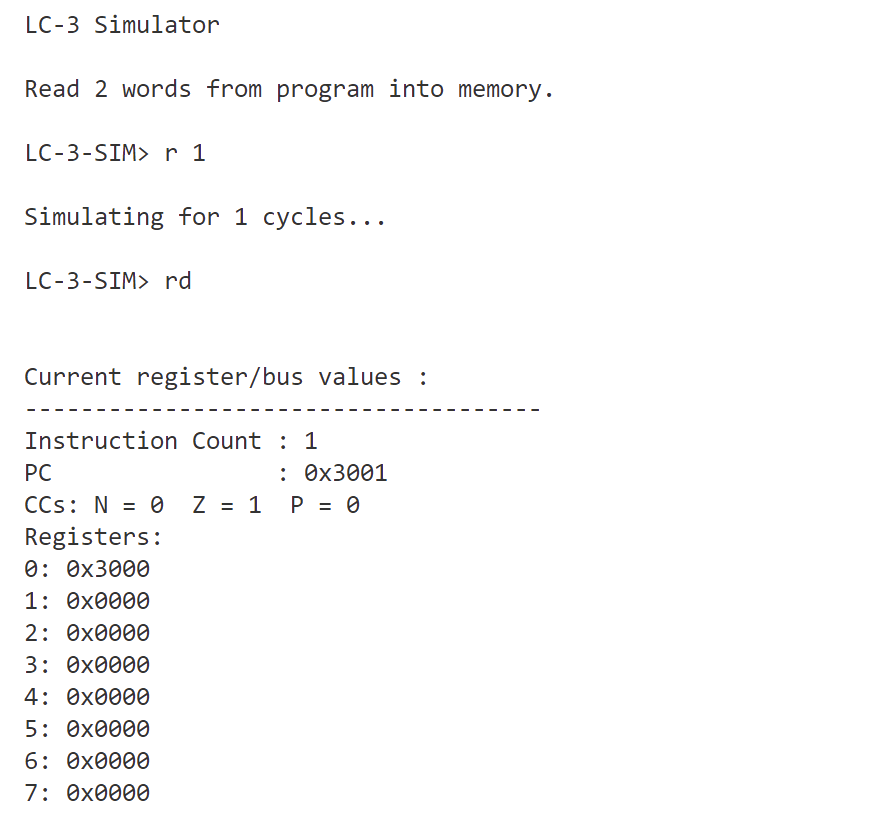
\includegraphics[width=\linewidth]{lea.png}
    \caption{LEA功能测试}
  \end{subfigure}
  \hfill
  \begin{subfigure}{0.48\textwidth}
    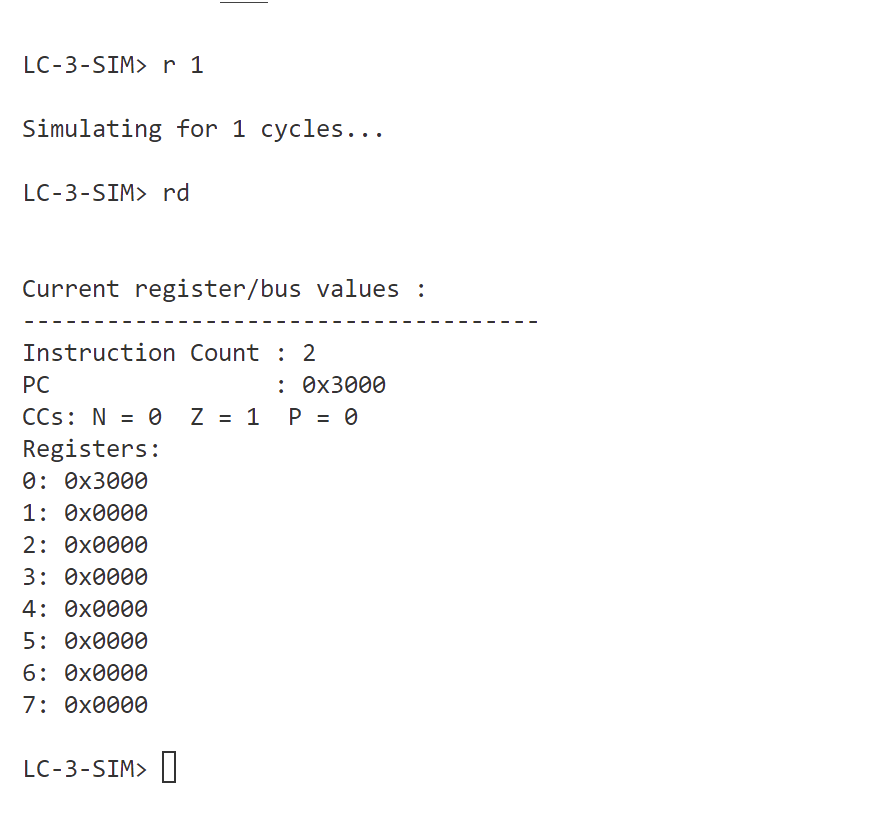
\includegraphics[width=\linewidth]{jmp.png}
    \caption{JMP功能测试}
  \end{subfigure}
  \caption{LEA与JMP功能测试}
  \label{leajmp}
\end{figure}

则LEA指令正确把地址加载到指定寄存器中,JMP正确跳转到对应寄存器中存储的地址,不改变条件码。由于RET指令就是JMP R7,后面不再单独测试。

\subsection{ST与LD功能测试}
运行如下代码:
\begin{enumerate}
  \item [ ] .ORIG 0x3000
  \item [0x3000] LEA R0,\# -1(0xE1FF)
  \item [0x3001] ST R0, \# 7(0x3007)
  \item [0x3002] LD R1, \#6(0x2206)
\end{enumerate}
运行结果如图\ref{stld}:
\begin{figure}[htbp]
  \centering
  \begin{subfigure}{0.48\textwidth} % 留出间距
    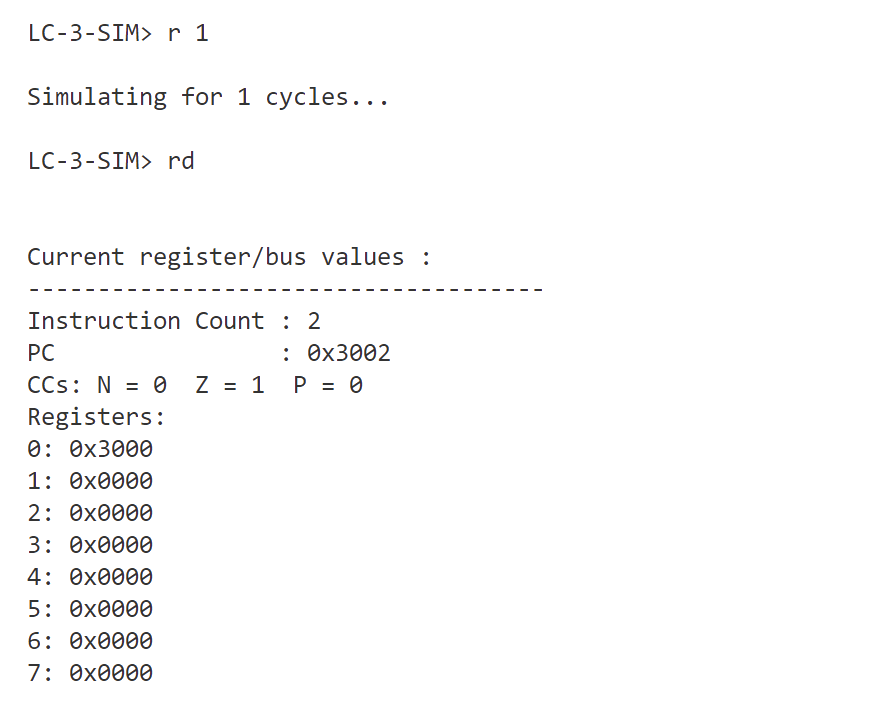
\includegraphics[width=\linewidth]{st.png}
    \caption{ST功能测试}
  \end{subfigure}
  \hfill
  \begin{subfigure}{0.48\textwidth}
    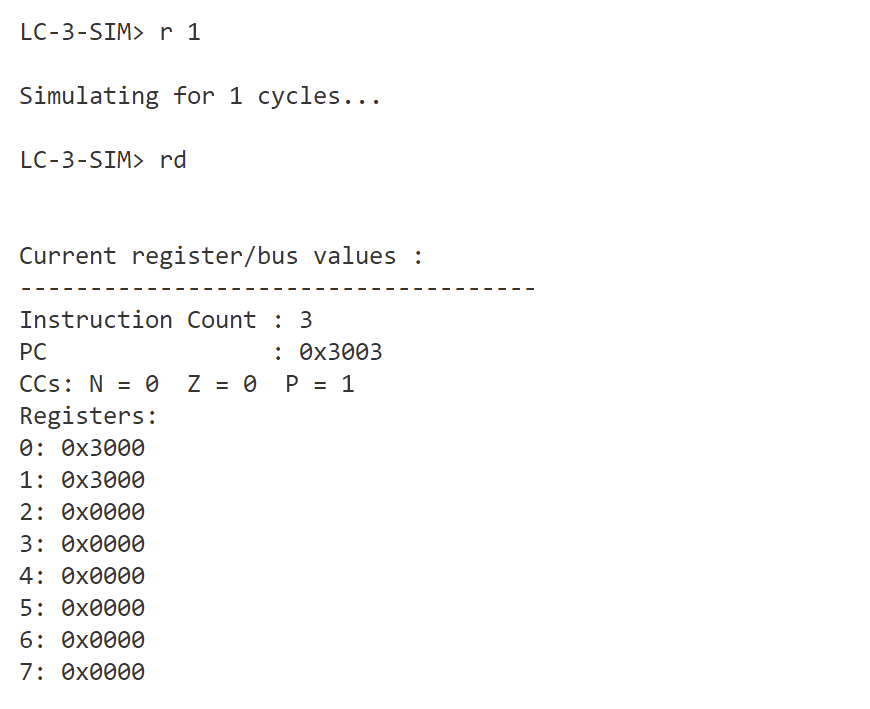
\includegraphics[width=\linewidth]{ld.png}
    \caption{LD功能测试}
  \end{subfigure}
  \caption{ST与LD功能测试}
  \label{stld}
\end{figure}
则ST指令正确把源寄存器的值存储到指定地址中,LD正确把数据加载到指定寄存器并设置条件码。

\subsection{STI与LDI功能测试}
由于全部初始化为0,所以STI和LDI都会访问0x0000.运行如下代码,使用mdump查看内存:
\begin{enumerate}
  \item [ ] .ORIG 0x3000
  \item [0x3000] ADD R0,R0,\# 1(0x1021)
  \item [0x3001] STI R0, \# 7(0xB007)
  \item [0x3002] LDI R1, \#6(0xA206)
\end{enumerate}
运行结果如图\ref{stildi}:
\begin{figure}[ht]
  \centering
  \begin{subfigure}{0.45\textwidth}
    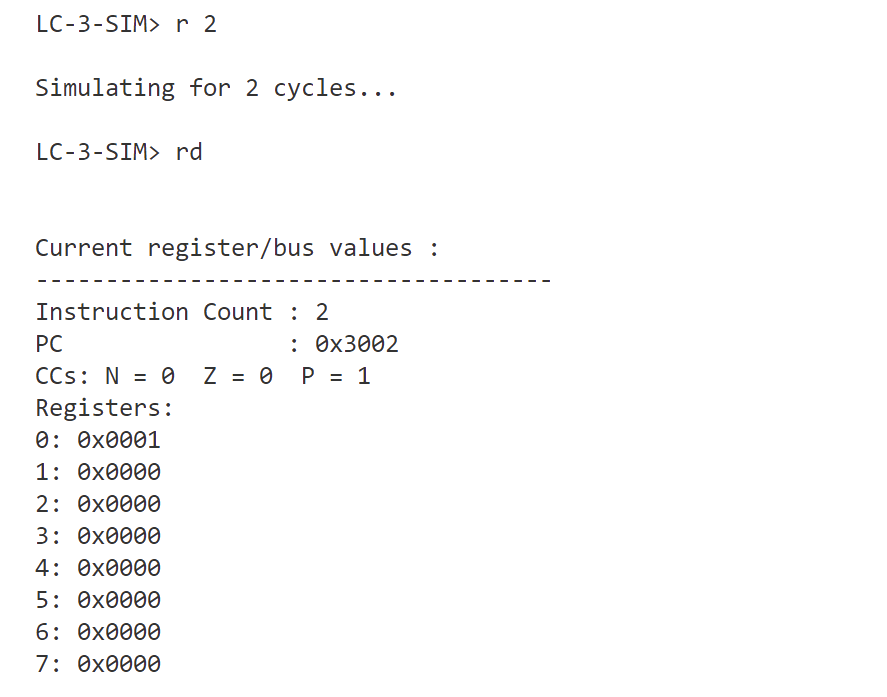
\includegraphics[width=\linewidth]{sti1.png}
    \caption{STI}
  \end{subfigure}
  \begin{subfigure}{0.45\textwidth}
    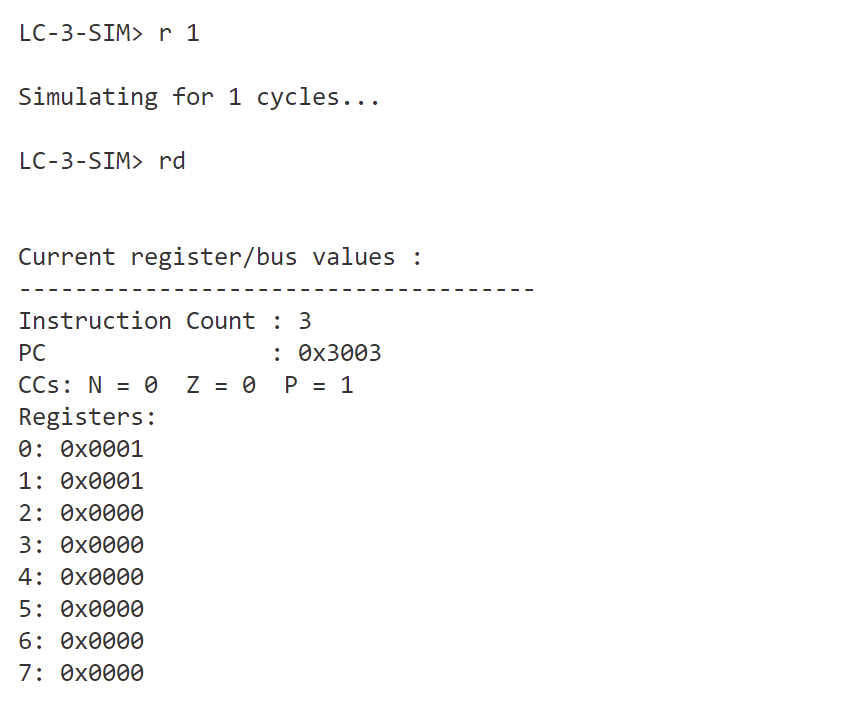
\includegraphics[width=\linewidth]{sti2.png}
    \caption{LDI}
  \end{subfigure}

  \begin{subfigure}{0.45\textwidth}
    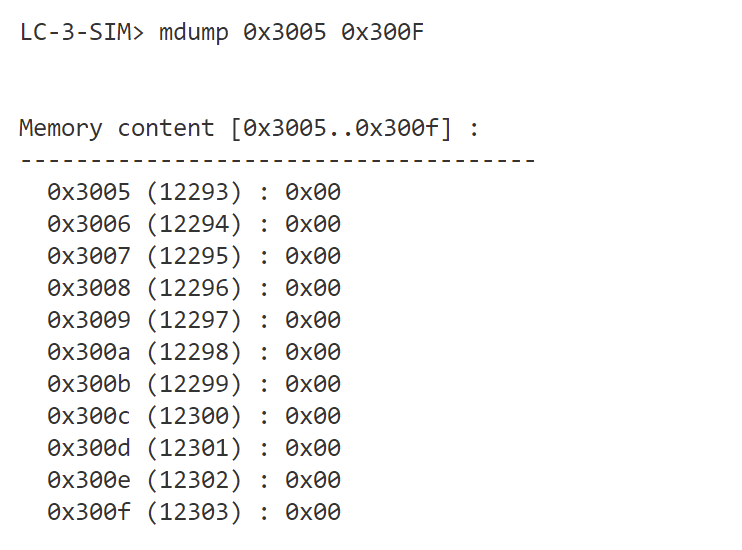
\includegraphics[width=\linewidth]{sti3.png}
    \caption{内存查看}
  \end{subfigure}
  \begin{subfigure}{0.44\textwidth}
    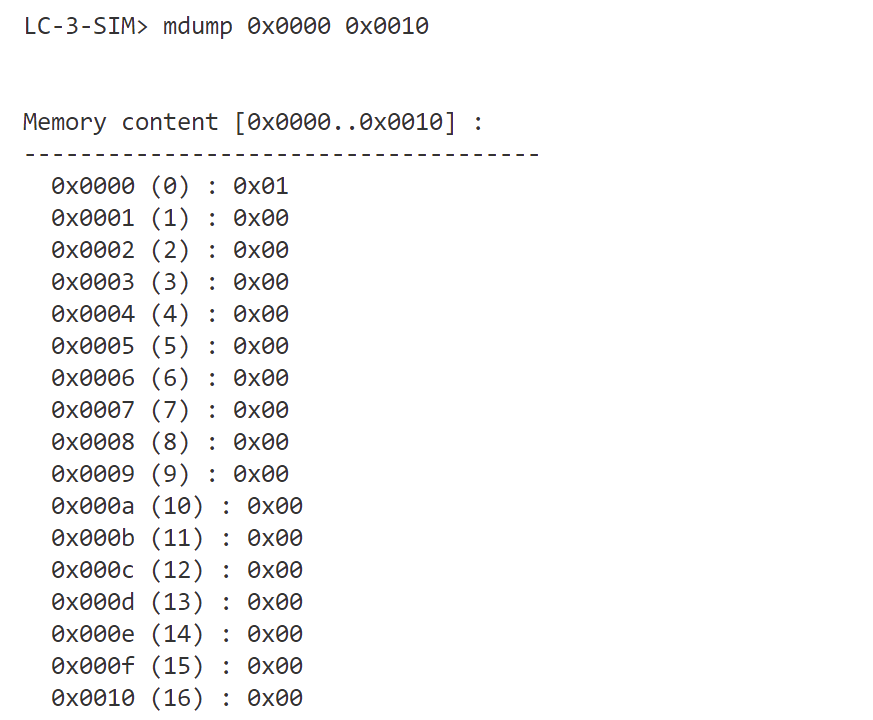
\includegraphics[width=\linewidth]{sti4.png}
    \caption{内存查看}
  \end{subfigure}
  \caption{STI与LDI功能测试}
  \label{stildi}
\end{figure}

则STI与LDI能正确存储与加载,且LDI正确设置条件码。

\subsection{STR与LDR功能测试}
运行如下代码,使用mdump查看内存.加入ADD R4,R4,\#1是为了改变条件码,便于对比查看。
\begin{enumerate}
  \item [ ] .ORIG 0x3000
  \item [0x3000] LEA R1,\# -1(0xE3FF)
  \item [0x3001] ADD R0,R0,\# -1(0x103F)
  \item [0x3002] ADD R4,R4,\#1(0x1921)
  \item [0x3003] STR R0,R1,\#7(0x7047)
  \item [0x3004] LDR R2,R1,\#7(0x6447)
\end{enumerate}
运行结果如图\ref{strldr}:
\begin{figure}[ht]
  \centering
  \begin{subfigure}{0.45\textwidth}
    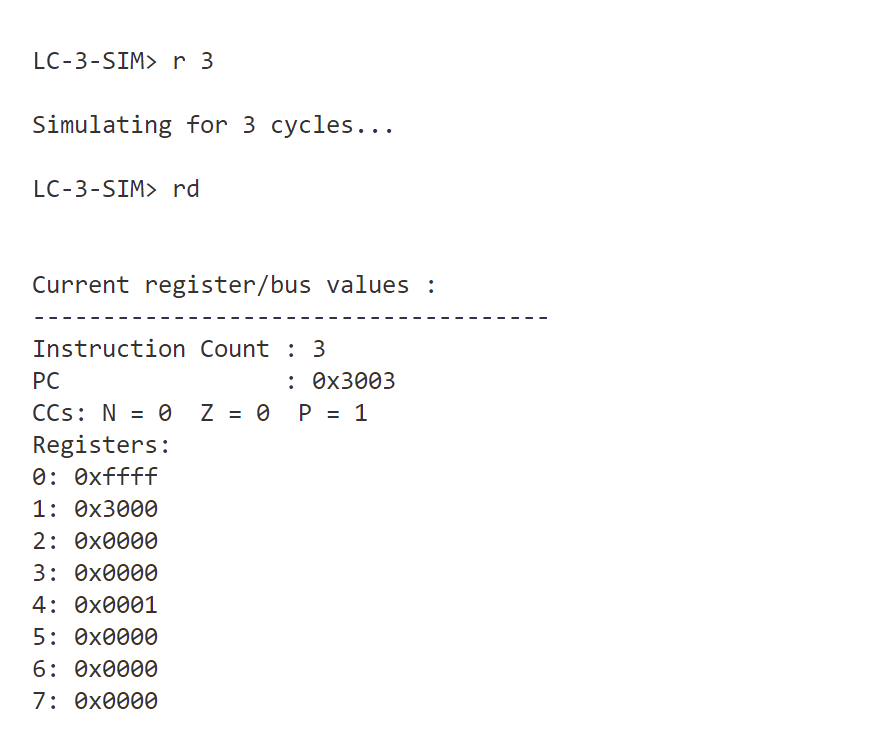
\includegraphics[width=\linewidth]{str1.png}
    \caption{前期准备}
  \end{subfigure}
  \begin{subfigure}{0.45\textwidth}
    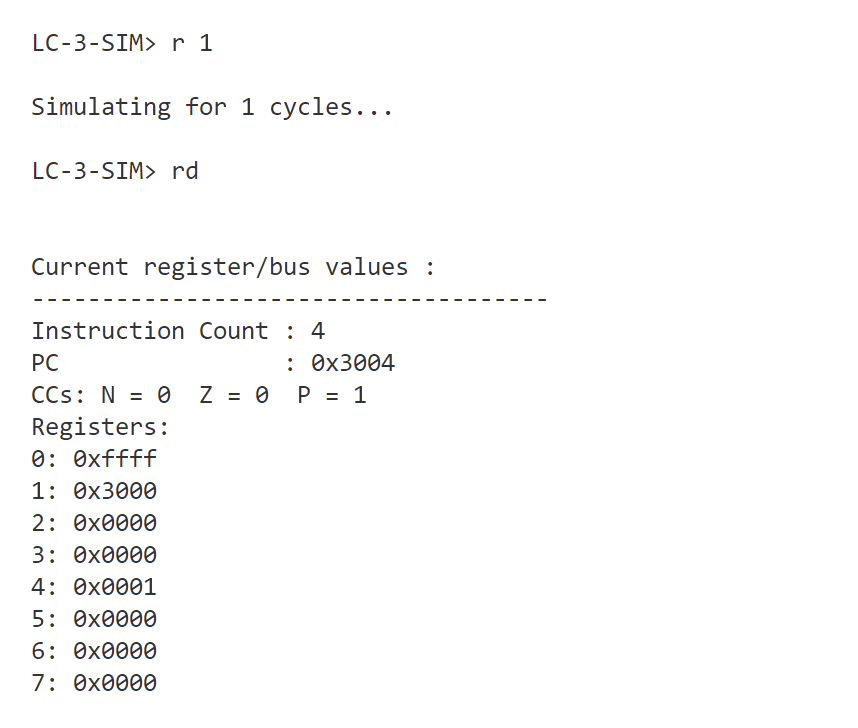
\includegraphics[width=\linewidth]{str2.png}
    \caption{STR}
  \end{subfigure}

  \begin{subfigure}{0.45\textwidth}
    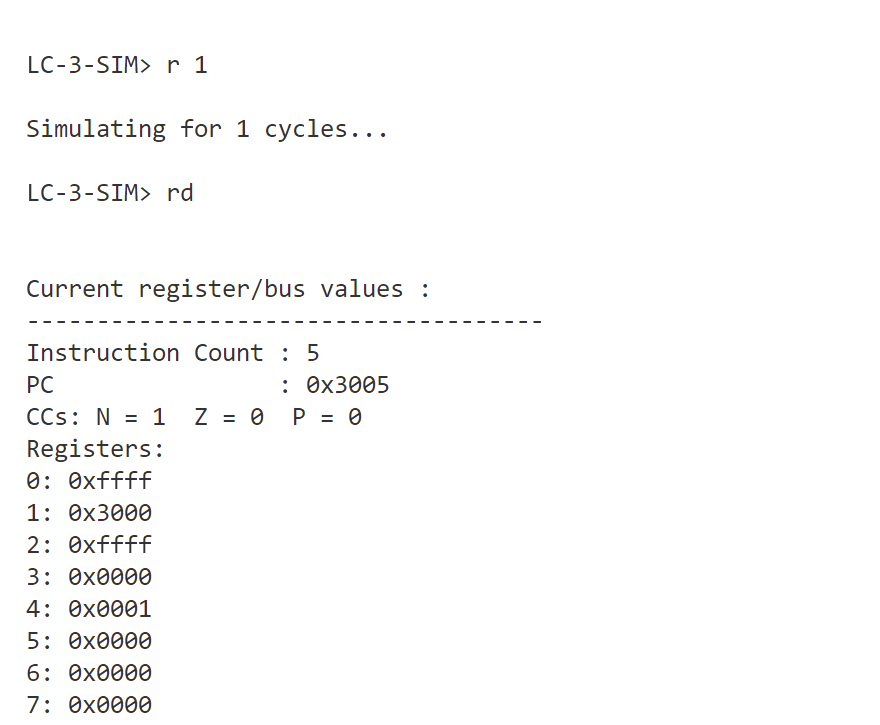
\includegraphics[width=\linewidth]{str3.png}
    \caption{LDR}
  \end{subfigure}
  \begin{subfigure}{0.44\textwidth}
    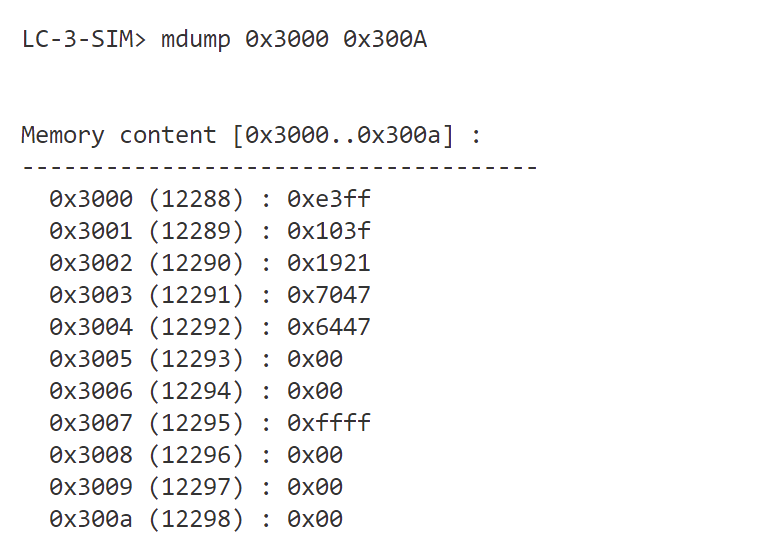
\includegraphics[width=\linewidth]{str4.png}
    \caption{内存查看}
  \end{subfigure}
  \caption{STR与LDR功能测试}
  \label{strldr}

\end{figure}

则STR与LDR能正确存储与加载,且LDR正确设置条件码。

\subsection{JSR与JSRR(与RET)功能测试}
执行以下命令,其中的BR是0x0000,无论如何不跳转,发挥NOP的作用。
\begin{enumerate}
  \item [ ] .ORIG 0x3000
  \item [0x3000] LEA R0,\# 5(0xE005)
  \item [0x3001] JSR \#3(0x4803)
  \item [0x3002] JSRR R0(0x4000)
  \item [0x3003] BR(0x0000)
  \item [0x3004] BR(0x0000)
  \item [0x3005] RET(0xC1C0)
  \item [0x3006] RET(0xC1C0)
\end{enumerate}
运行结果如图:
\begin{figure}[htbp]
  \centering
  \begin{subfigure}{0.45\textwidth}
    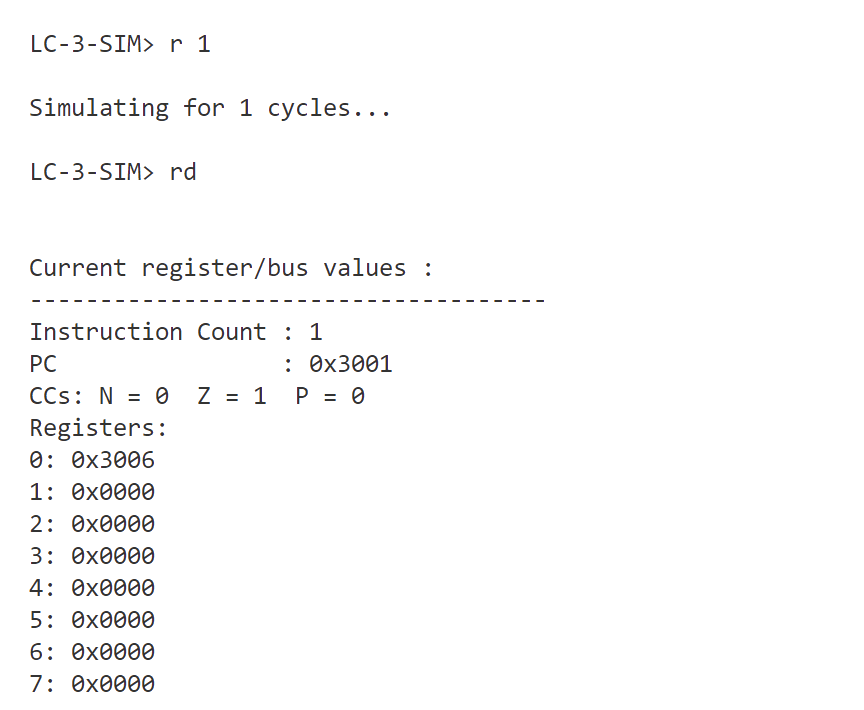
\includegraphics[width=\linewidth]{jsr1.png}
    \caption{准备工作}
  \end{subfigure}
  \hfill
  \begin{subfigure}{0.45\textwidth}
    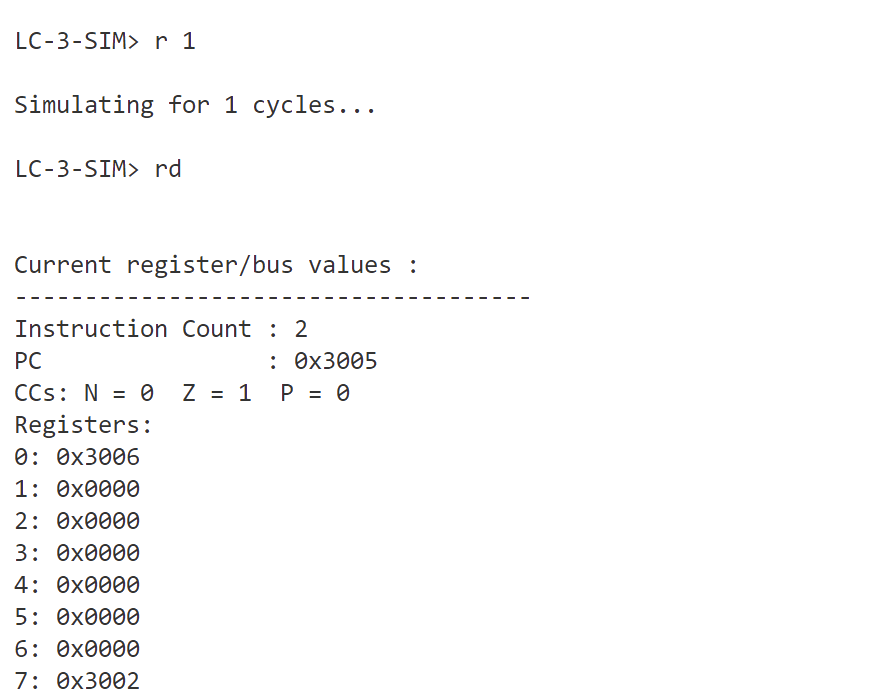
\includegraphics[width=\linewidth]{jsr2.png}
    \caption{JSR}
  \end{subfigure}

  \vspace{0.5cm}

  \begin{subfigure}{0.45\textwidth}
    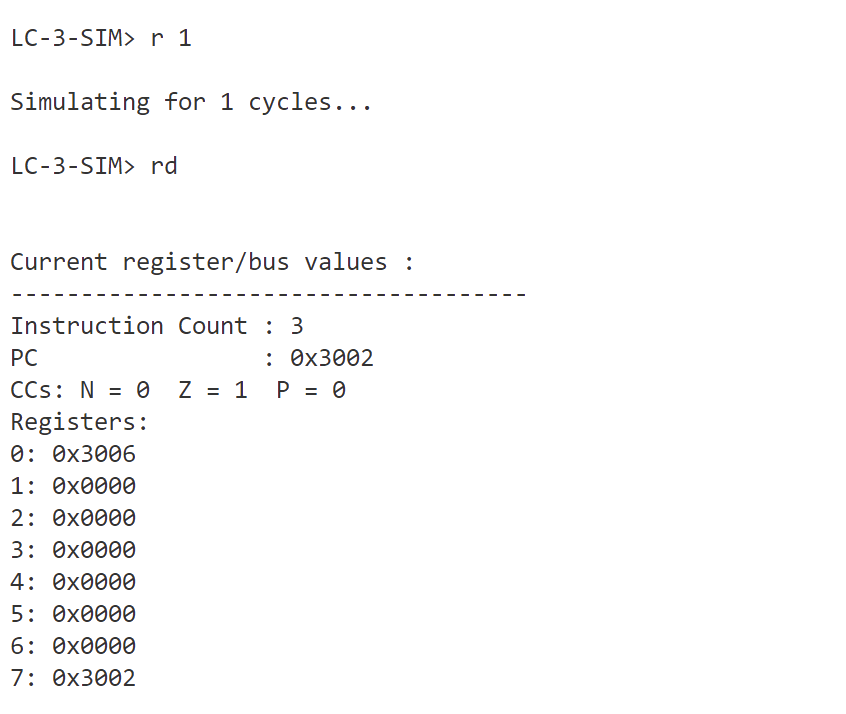
\includegraphics[width=\linewidth]{jsr3.png}
    \caption{RET}
  \end{subfigure}
  \hfill
  \begin{subfigure}{0.45\textwidth}
    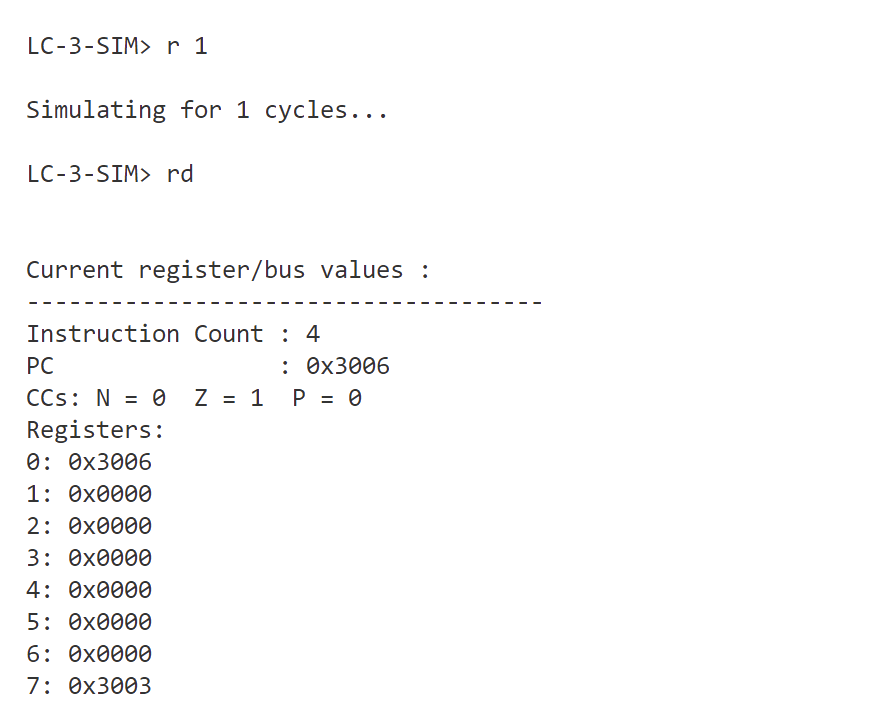
\includegraphics[width=\linewidth]{jsr4.png}
    \caption{JSRR}
  \end{subfigure}

  \vspace{0.5cm}

  \begin{subfigure}{0.45\textwidth}
    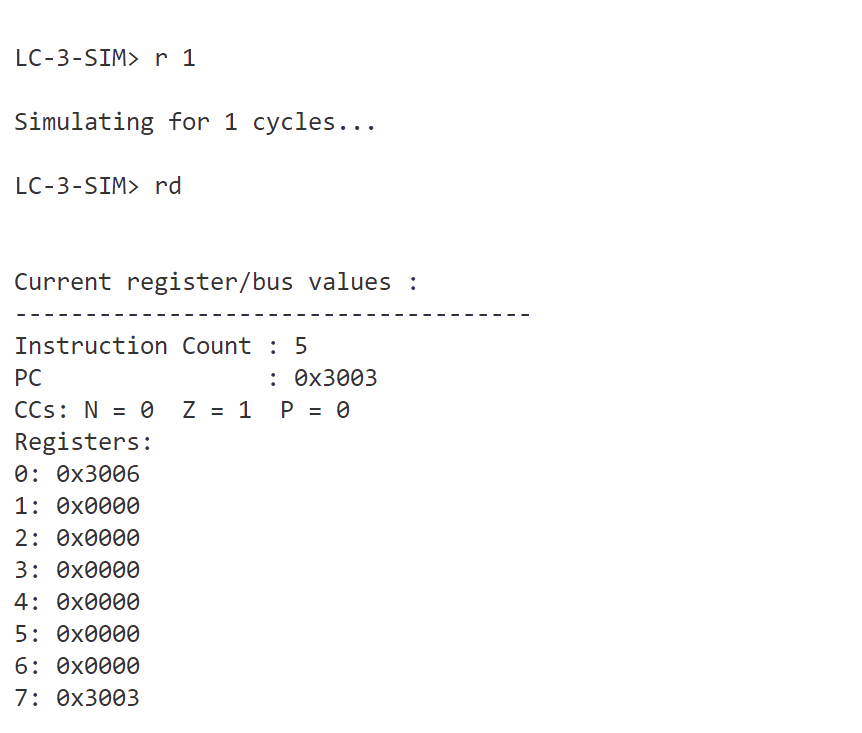
\includegraphics[width=\linewidth]{jsr5.png}
    \caption{RET}
  \end{subfigure}
  \hfill
  \begin{subfigure}{0.45\textwidth}
    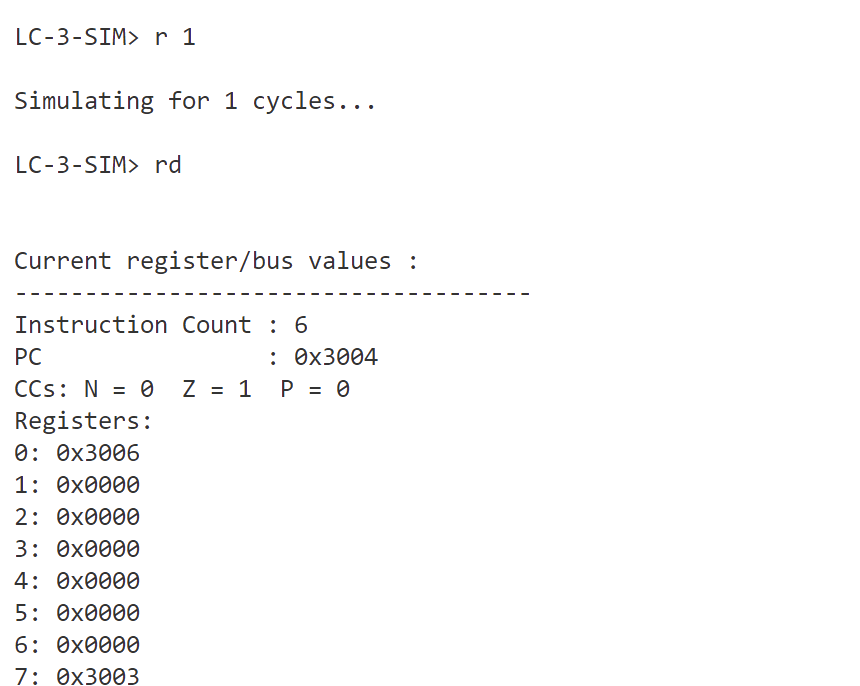
\includegraphics[width=\linewidth]{jsr6.png}
    \caption{顺序执行}
  \end{subfigure}

  \caption{JSR与JSRR(与RET)功能测试}
  \label{jsr}
  则JSR,JSRR可以正确跳转并保存自增后的PC到R7,RET可以正确返回。
\end{figure}

\subsection{总结}
总而言之,ADD,NOT,AND,BR,TRAP,LEA,JMP,ST,LD,STI,LDT,STR,LDR,JSR指令在各个模式下均工作正常。




\end{document}